\begin{figure}[htp]
  \centering
  \begin{tikzpicture}
    \begin{axis}[width=\textwidth, height=6cm, ylabel=Absorptionsrate, xlabel=Wellenlänge $\lambda$ in \si{\micro\metre},xmin=1500, xmax=17750, legend cell align={left}, scaled x ticks={real:1000}, xtick scale label code/.code={}, ymin=-1, ymax=2.5]
      \addplot[blue, thick] table[x index=0,y index=4, col sep=semicolon]{Daten/AbsorptionSiO2.csv};
      \addlegendentry{mit Dotierung}
      \addplot[orange, thick] table[x index=0,y index=5, col sep=semicolon]{Daten/AbsorptionSiO2.csv};
      \addlegendentry{ohne Dotierung}
    \end{axis}
  \end{tikzpicture}
  \caption{Verhältnis des jeweiligen Signals zum Referenzsignal.}
  \label{fig:AbsorptionsrateSiO2}
\end{figure}

% \begin{figure}[htp]
%   \centering
%     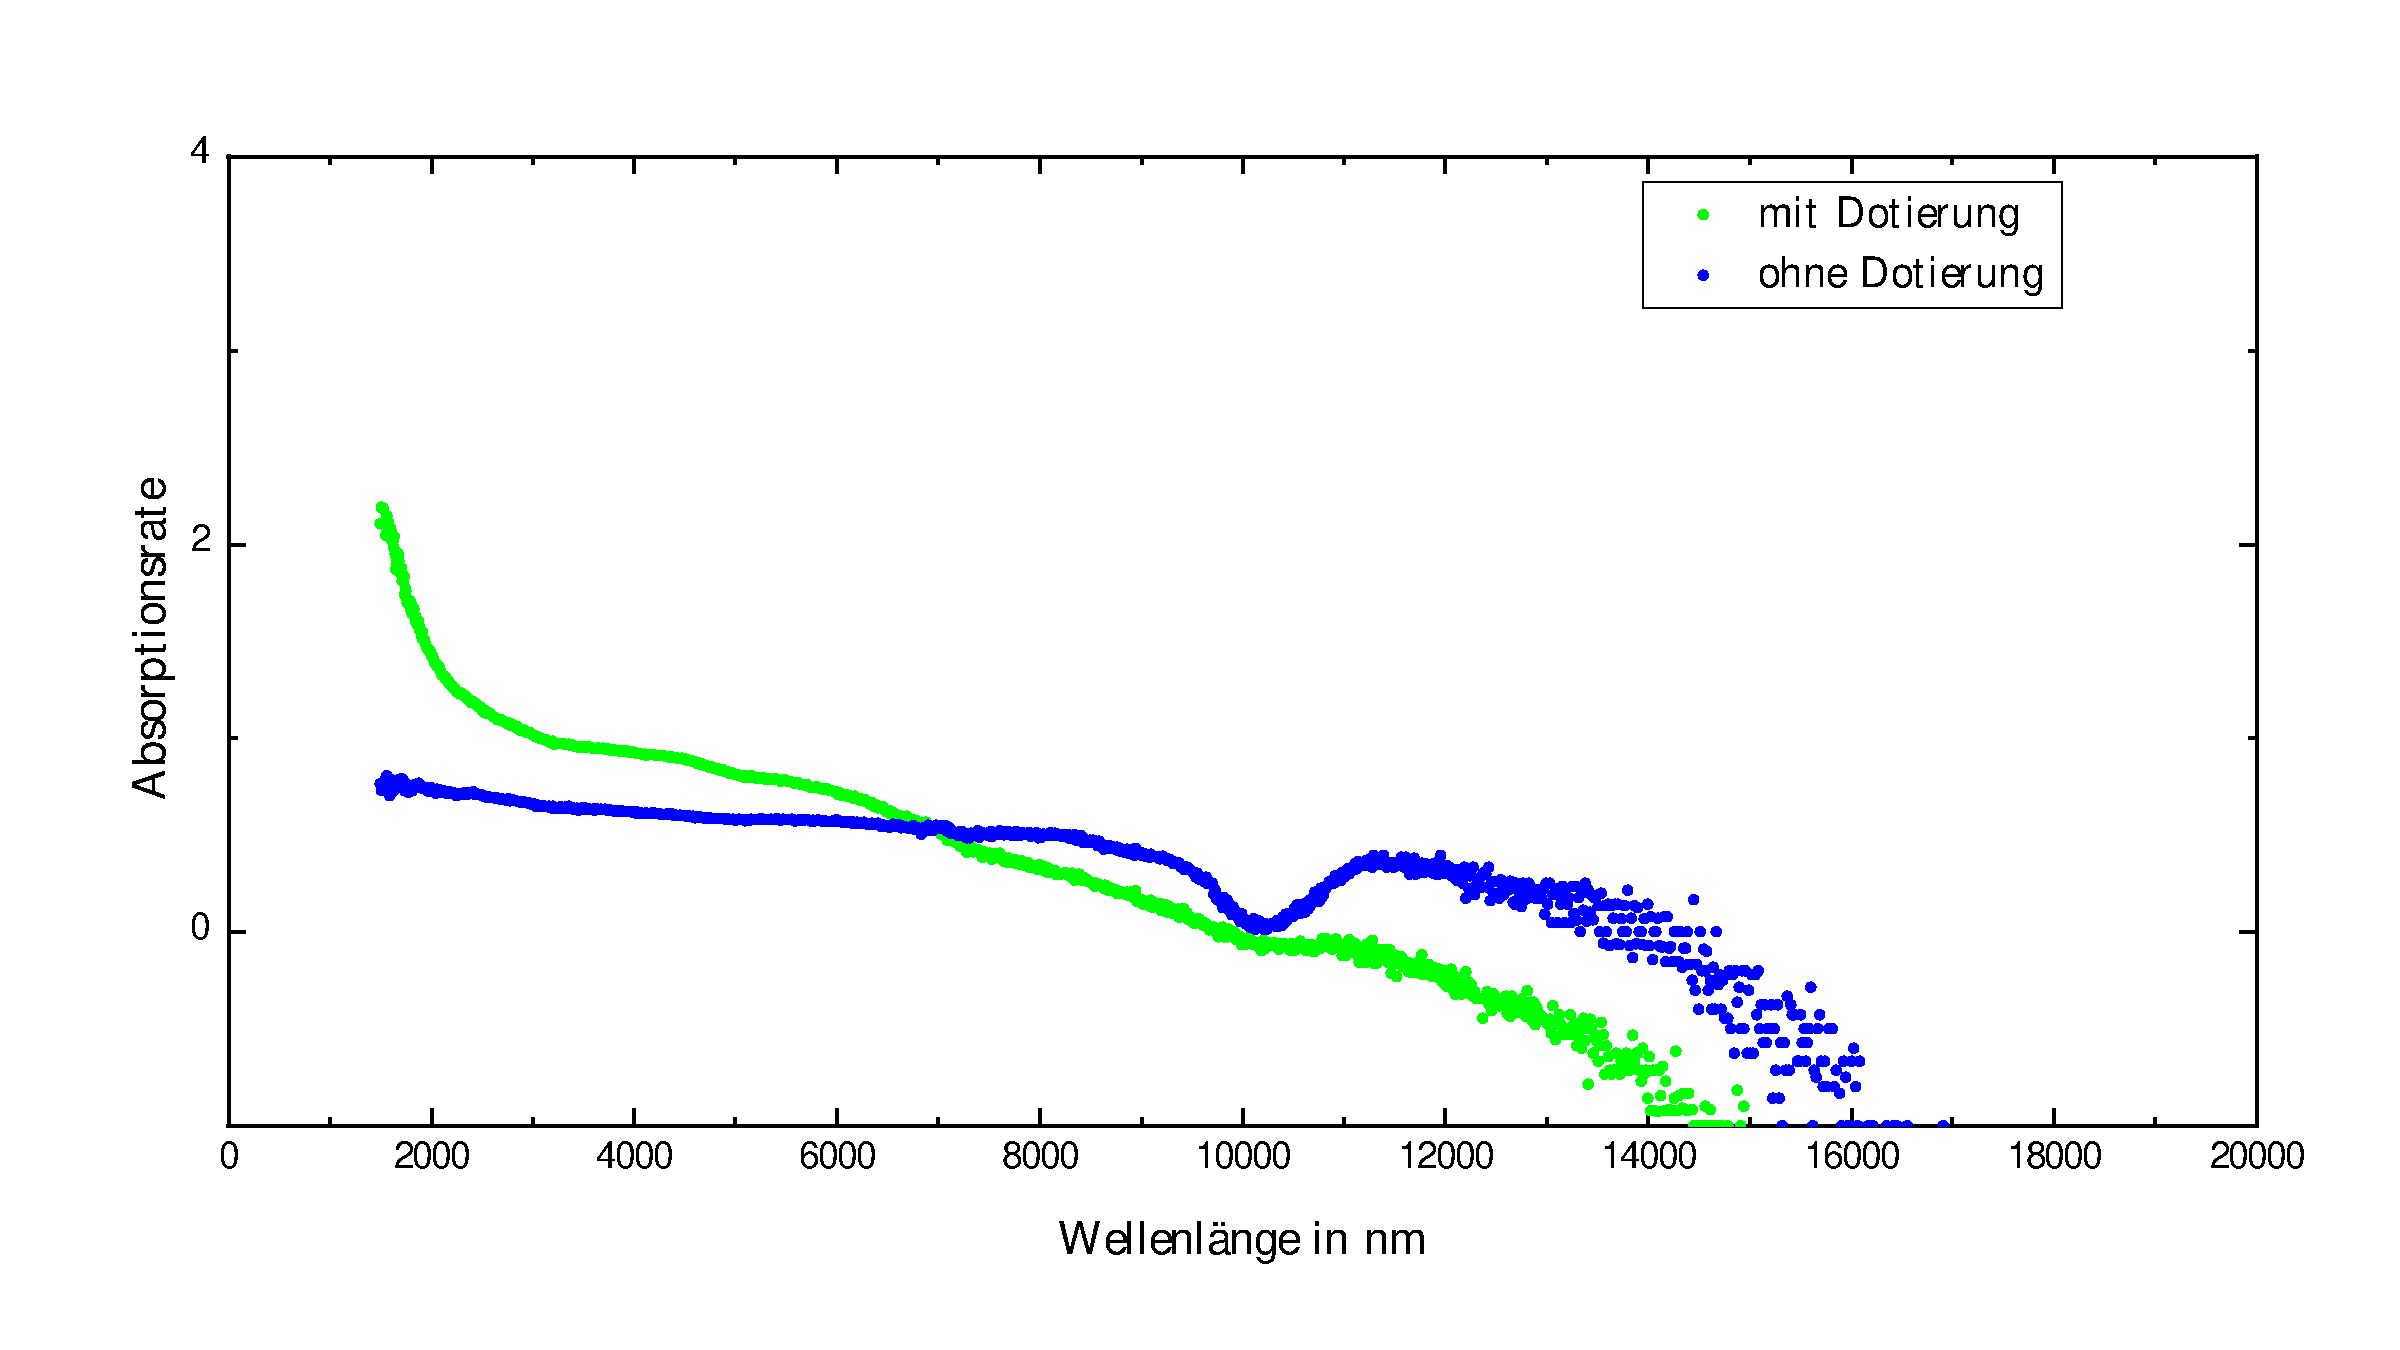
\includegraphics[width=\textwidth]{Bilder/Absorptionsrate_Si02.pdf}
%     \caption{Verhältnis jeweiliges Signal zu Referenzsignal}
% \end{figure}
